\section{Hamilton Arrives: Symplectic Elegance and Canonical Insight (1833)}

\subsection{Hamilton’s Leap: From Lagrange’s Velocities to Hamilton’s Momentums}

Lagrange had shown that the motion of a mechanical system could be reduced to a system of second-order differential equations involving positions \( q_i \), their time derivatives \( \dot{q}_i \), and a function \( L(q_i, \dot{q}_i, t) \), the Lagrangian:
\[
\frac{d}{dt} \left( \frac{\partial L}{\partial \dot{q}_i} \right) - \frac{\partial L}{\partial q_i} = 0
\]

This was a triumph: mechanics no longer needed forces or vectors—just energy and calculus. It was a world governed by optimization—by nature’s preference for efficient paths.

But Lagrange’s method still bundled position and velocity into a single evolving equation. It worked—but Hamilton saw something deeper.

\vspace{1em}
\textbf{What if position and motion were treated separately?}

Instead of describing motion solely in terms of position \( q_i \) and its rate \( \dot{q}_i \), Hamilton introduced a new variable: the \emph{conjugate momentum}:
\[
p_i = \frac{\partial L}{\partial \dot{q}_i}
\]

This momentum wasn’t an afterthought—it became a core coordinate of the system. With it, Hamilton re-expressed Lagrange’s mechanics as a pair of \emph{first-order} equations.

\subsubsection*{A Shift in Philosophy}

Lagrange was very much a product of the Enlightenment: he wanted to express nature’s laws as the consequence of a single, rational principle—least action. His world was deterministic, orderly, and elegant.

But Hamilton’s project came at a turning point. Though still shaped by Enlightenment ideals, his thinking was more romantic, more structural. He was less interested in describing nature’s \textit{path} and more in revealing its \textit{architecture}. He believed in a hidden symphony beneath motion—something richer than optimization, something geometric.

\textbf{Where Lagrange optimized a journey, Hamilton mapped a terrain.}

Hamilton was also a deeply spiritual thinker, heavily influenced by classical metaphysics and idealism. He believed that mathematics could reveal not just the behavior of nature, but the deep symmetry of its form. His work sought not merely to describe the world, but to encode it—like writing the score to a cosmic symphony in which every note (position) was accompanied by a harmony (momentum).

\vspace{1em}
\textbf{The Transformation That Changed Everything}

Hamilton’s key move was a transformation of variables—a kind of mathematical pivot. Starting from the Lagrangian \( L(q_i, \dot{q}_i, t) \), he defined a new function, now called the \emph{Hamiltonian}:
\[
H(q_i, p_i, t) = \sum_i p_i \dot{q}_i - L(q_i, \dot{q}_i, t)
\]

This function often corresponded to the total energy of the system. But Hamilton didn’t treat it as an energy calculator—he used it as a rulebook. The evolution of the system was now governed by these equations:
\[
\dot{q}_i = \frac{\partial H}{\partial p_i}, \qquad \dot{p}_i = -\frac{\partial H}{\partial q_i}
\]

No more second-order differentials. No acceleration. Just positions and momenta, each evolving in time through first-order derivatives.

\vspace{1em}
\textbf{Why This Mattered}

Hamilton’s equations weren’t just notational sleight of hand. They gave:

\begin{itemize}
    \item A new way to solve problems that Lagrange’s method struggled with.
    \item A symmetric formulation—each equation had a mirror.
    \item A powerful new language for expressing conservation laws.
    \item A geometric structure—what we now call \textbf{symplectic geometry}—with deep ties to modern physics.
\end{itemize}

Where Lagrange’s method asked how positions changed with time, Hamilton’s asked how position and momentum \emph{jointly} evolved, step by step. This provided a clearer path from the equations of motion to the conserved quantities hidden within them.

\vspace{1em}
\subsubsection*{From Enlightenment to Structure: Hamilton’s Philosophy}

Hamilton didn’t abandon the Enlightenment dream of determinism—but he reframed it.

Lagrange gave us a universe ruled by preference (least action). Hamilton gave us a universe ruled by \textbf{structure}—one that moved not just with direction but with rhythm. His equations didn’t just predict—they revealed a hidden grammar, a \textbf{canonical form} of reality.

Where Newton had asked "What causes what?" and Lagrange asked "What path minimizes action?", Hamilton asked:
\begin{quote}
    \emph{What is the underlying geometry of motion itself?}
\end{quote}

His answer wasn’t just a reformulation—it was a revelation. The separation of position and momentum, encoded in the Hamiltonian framework, would become the foundation of quantum mechanics, statistical physics, and beyond.

\begin{quote}
\textit{Lagrange made motion a question of calculus.  
Hamilton made it a system—structured, separable, and ready for generalization.}
\end{quote}

\begin{figure}[H]
  \centering
  
  % === First row ===
  \begin{subfigure}[t]{0.45\textwidth}
  \centering
  \begin{tikzpicture}
    \comicpanel{0}{0}
      {Lagrange}
      {}
      {I turned Newton’s mechanics into a clean calculus problem. No forces. No diagrams. Just elegance.}
      {(0,-0.6)}
  \end{tikzpicture}
  \caption*{Lagrange: Optimization is nature’s compass.}
  \end{subfigure}
  \hfill
  \begin{subfigure}[t]{0.45\textwidth}
  \centering
  \begin{tikzpicture}
    \comicpanel{0}{0}
      {Hamilton}
      {}
      {Lovely. But what if motion is a symphony, and we’re missing the sheet music?}
      {(0,-0.6)}
  \end{tikzpicture}
  \caption*{Hamilton: Structure is nature’s score.}
  \end{subfigure}
  
  \vspace{1em}
  
  % === Second row ===
  \begin{subfigure}[t]{0.45\textwidth}
  \centering
  \begin{tikzpicture}
    \comicpanel{0}{0}
      {Lagrange}
      {}
      {Minimize the action. That’s the rule. Simple, universal, deterministic.}
      {(0,0.8)}
  \end{tikzpicture}
  \caption*{Lagrange: Let nature choose the most efficient path.}
  \end{subfigure}
  \hfill
  \begin{subfigure}[t]{0.45\textwidth}
  \centering
  \begin{tikzpicture}
    \comicpanel{0}{0}
      {Hamilton}
      {}
      {Let nature evolve in phase space. It’s not just a path—it’s a map.}
      {(0,0.8)}
  \end{tikzpicture}
  \caption*{Hamilton: Let geometry do the talking.}
  \end{subfigure}
  
  \caption{Lagrange saw motion as a question of calculus. Hamilton saw it as the unfolding of deep structure.}
  \end{figure}






  
  
  \subsection{The Hamiltonian Method: From Motion to Phase Space}

  Hamilton’s contribution wasn’t a rejection of Lagrange—it was a deeper structural refinement. Where Lagrange described motion using positions \( q_i \) and their time derivatives \( \dot{q}_i \), Hamilton recast the story in terms of \textbf{phase space}—a new way of thinking about the state of a system.
  
  \textbf{Configuration space} is what Lagrange used: it tracks only the positions of a system’s components. If you’re describing a pendulum, for instance, configuration space tells you the angle of the bob.
  
  But Hamilton asked a new question:
  \begin{quote}
      \textit{What if we tracked both where a system is, and how it's moving?}
  \end{quote}
  
  This led to the idea of \textbf{phase space}, which tracks both positions \( q_i \) and momenta \( p_i \) as independent variables. Instead of describing the shape of a system’s trajectory (as in configuration space), phase space describes the \textit{state} of the system completely.
  
  \begin{center}
    \begin{tabularx}{\textwidth}{|c|X|X|}
    \hline
    \textbf{Concept} & \textbf{Configuration Space} & \textbf{Phase Space} \\
    \hline
    What it tracks & Positions (\( q_1, q_2, \dots \)) & Positions and Momenta (\( q_i, p_i \)) \\
    \hline
    Example Coordinate & \( q = x \) & \( (q, p) = (x, p_x) \) \\
    \hline
    Analogy & GPS map: shows where you are & Dashboard: shows where you are and how fast you're moving \\
    \hline
    Purpose & Describes shape or configuration & Describes full dynamical state \\
    \hline
    Time Evolution & Needs second derivatives (e.g., acceleration) & Evolves via first-order flows \\
    \hline
    \end{tabularx}
    \end{center}
    
  
  \vspace{1em}
  \textbf{Intuition:}
  
  Imagine you're watching a planet orbit the Sun:
  
  - In \textbf{configuration space}, you trace the path the planet makes across the sky—a map of where it is at each moment.
  - In \textbf{phase space}, you see not only the planet’s location but also its speed and direction at every point—a complete snapshot of its motion.
  
  Here’s the key:
  \begin{quote}
      \textit{The same location can appear multiple times in configuration space—but in phase space, each state is unique.}
  \end{quote}
  
  That uniqueness made phase space a more powerful language for dynamics.
  
  \vspace{1em}
  
  \textbf{Hamilton formalized this with mathematics.} Given a Lagrangian \( L(q, \dot{q}, t) \), he defined the conjugate momentum:
  \[
  p_i = \frac{\partial L}{\partial \dot{q}_i}
  \]
  
  Then, performing a Legendre transform, he introduced the \textbf{Hamiltonian}:
  \[
  H(q, p, t) = \sum_i p_i \dot{q}_i - L(q, \dot{q}, t)
  \]
  
  This function often corresponds to the total energy of the system. But more importantly, Hamilton used it to create a new set of equations that govern how both \( q_i \) and \( p_i \) evolve in time:
  \[
  \dot{q}_i = \frac{\partial H}{\partial p_i}, \qquad \dot{p}_i = -\frac{\partial H}{\partial q_i}
  \]
  
  These are \textbf{first-order equations}—no acceleration, no forces, just flows through phase space.
  
  \begin{quote}
      \textit{In Lagrangian mechanics, motion was a path. In Hamiltonian mechanics, motion became a flow—through a geometric landscape of possibilities.}
  \end{quote}


  \begin{figure}[H]
    \centering
    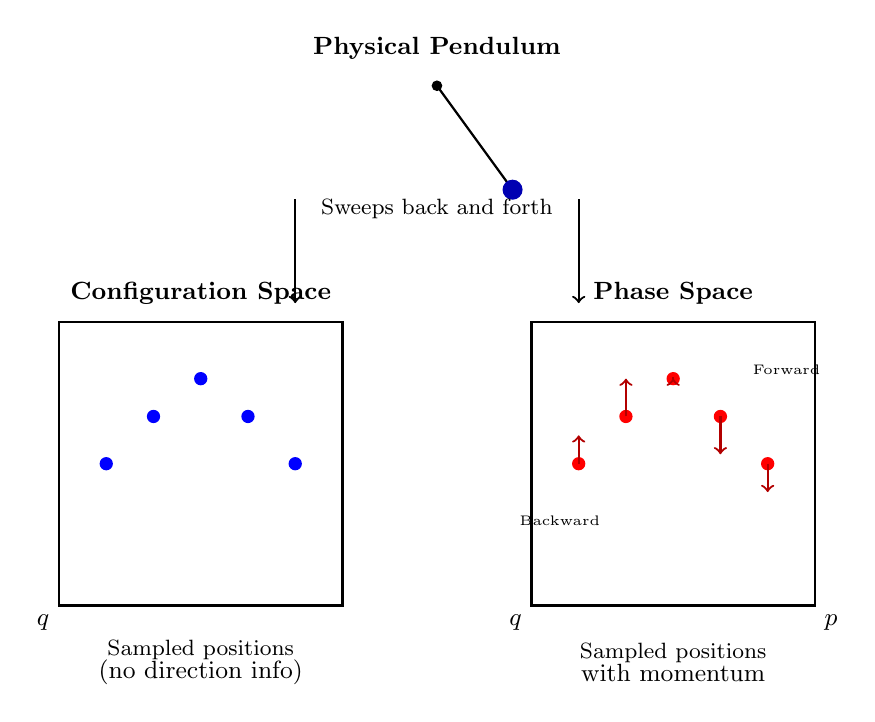
\begin{tikzpicture}[scale=1.2, every node/.style={font=\small}]
    
      % === Pendulum Above Boxes ===
      \draw[fill=black] (5,5.5) circle (0.05cm); % pivot
      \draw[thick] (5,5.5) -- (5.8,4.4);         % rod
      \filldraw[blue!70!black] (5.8,4.4) circle (0.1cm); % bob
      \node at (5,5.9) {\textbf{Physical Pendulum}};
      \node at (5,4.2) {\footnotesize Sweeps back and forth};
    
      % Arrows down to boxes
      \draw[->, thick] (3.5,4.3) -- (3.5,3.2);
      \draw[->, thick] (6.5,4.3) -- (6.5,3.2);
    
      % === Configuration Space ===
      \draw[thick] (1,0) rectangle (4,3);
      \node at (2.5,3.3) {\textbf{Configuration Space}};
      \node at (1,0) [below left] {\(q\)};
      \node at (2.5,-0.6) [align=center] {\footnotesize Sampled positions\\[-0.3em] (no direction info)};
    
      % 5 sample positions (no direction)
      \foreach \x/\y in {1.5/1.5, 2/2, 2.5/2.4, 3/2, 3.5/1.5} {
        \fill[blue] (\x,\y) circle (2pt);
      }
    
      % === Phase Space ===
      \begin{scope}[shift={(5,0)}]
        \draw[thick] (1,0) rectangle (4,3);
        \node at (2.5,3.3) {\textbf{Phase Space}};
        \node at (1,0) [below left] {\(q\)};
        \node at (4,0) [below right] {\(p\)};
        \node at (2.5,-0.6) [align=center] {\footnotesize Sampled positions\\[-0.3em] with momentum};
    
        % 5 sample positions with arrows
        \foreach \x/\y/\dx/\dy in {
          1.5/1.5/0/0.3,
          2/2/0/0.4,
          2.5/2.4/0/0,
          3/2/0/-0.4,
          3.5/1.5/0/-0.3
        } {
          \fill[red] (\x,\y) circle (2pt);
          \draw[->, thick, red!70!black] (\x,\y) -- ++(\dx,\dy);
        }
    
        % Optional: annotate direction
        \node at (3.7,2.5) {\tiny Forward};
        \node at (1.3,0.9) {\tiny Backward};
      \end{scope}
    
    \end{tikzpicture}
    \caption{Configuration space (left) shows sampled positions of the pendulum. Phase space (right) includes both position and momentum—capturing the system’s full dynamic state.}
    \end{figure}
    

    
    \begin{tcolorbox}[colback=blue!5!white, colframe=blue!50!black, 
      title={Historical Sidebar: Kant’s Philosophy and the Mechanics of Thought}]
      
          \textbf{Immanuel Kant} (1724–1804) never wrote a treatise on classical mechanics, but his philosophy quietly reshaped the intellectual foundation beneath it. In his \textit{Critique of Pure Reason}, Kant argued that \textbf{space and time are not features of the external world}, but \textbf{forms of human intuition}—the lenses through which we structure all experience.
      
          \medskip
      
          This radical idea—that the mind imposes order on the chaos of sensation—profoundly influenced later thinkers who wanted to understand not just what nature does, but \textbf{how we come to know it}. Among them was the Irish mathematician and physicist \textbf{William Rowan Hamilton}, who internalized Kant’s metaphysics and applied it to physics.
      
          \medskip
      
          Hamilton’s work in analytical mechanics wasn’t just about refining Newton—it was about expressing the laws of motion in a way that mirrored the rational structure of thought. He viewed his equations not just as descriptions of forces, but as revelations of the deep symmetry between \textbf{how the mind perceives change} and how systems evolve in time.
      
          \medskip
      
          In this sense, Hamiltonian mechanics became a kind of applied Kantianism: a precise, mathematical language for modeling causality, time, and motion from the inside out. It foreshadowed the structure of quantum mechanics, where the observer, system, and measurement become inseparable.
      
          \medskip
      
          \textbf{Quote from Hamilton (1835):}
          \begin{quote}
          “The science of time is algebra... the progress of the mind in symbol is analogous to the flow of nature in law.”
          \end{quote}
      
          Kant gave the Enlightenment a new model of the mind. Hamilton translated that model into motion—turning metaphysics into mechanics.
          
      \end{tcolorbox}
      
      
    
  

\subsection{Kepler Redux: The Second Law in Hamilton’s World}

In Lagrange’s method, conservation laws emerged from symmetries in the coordinates. In Hamilton’s formulation, they arise from invariances in the \emph{structure} of phase space. If a coordinate \( q_i \) is cyclic—meaning \( H \) does not depend on it—then its conjugate momentum \( p_i \) is conserved:
\[
\frac{\partial H}{\partial q_i} = 0 \quad \Rightarrow \quad \dot{p}_i = 0
\]

Consider again planetary motion in two generalized coordinates:
\begin{itemize}
  \item \( q_1 \): radial distance
  \item \( q_2 \): angular coordinate
\end{itemize}

The Lagrangian was:
\[
L = \frac{1}{2} m \left( \dot{q}_1^2 + a(q_1)^2 \dot{q}_2^2 \right) - V(q_1)
\]
Compute the conjugate momenta:
\[
p_1 = \frac{\partial L}{\partial \dot{q}_1} = m \dot{q}_1, \qquad
p_2 = \frac{\partial L}{\partial \dot{q}_2} = m a(q_1)^2 \dot{q}_2
\]

The Hamiltonian becomes:
\[
H(q_1, q_2, p_1, p_2) = \frac{p_1^2}{2m} + \frac{p_2^2}{2m a(q_1)^2} + V(q_1)
\]

Since \( q_2 \) does not appear in \( H \), it is a cyclic coordinate. Therefore, \( \dot{p}_2 = -\frac{\partial H}{\partial q_2} = 0 \), and angular momentum \( p_2 \) is conserved:
\[
p_2 = m a(q_1)^2 \dot{q}_2 = \text{const}
\]

Which again leads to:
\[
\frac{dA}{dt} \propto a(q_1)^2 \dot{q}_2 = \text{const}
\quad \Rightarrow \quad \text{Kepler’s Second Law}
\]

\subsubsection{Phase Space and Symplectic Structure}

Hamilton didn’t just rewrite the equations of motion — he reimagined the stage on which motion takes place. Instead of thinking only in terms of positions and how they change, he introduced a new framework: \textbf{phase space}, where every state of a system is described not just by its coordinates \( q_i \), but also by their corresponding momenta \( p_i \). These pairs form the fundamental building blocks of Hamiltonian mechanics.

But Hamilton went further. He showed that this space wasn’t just a convenient way to organize variables — it had a deep geometric structure. He defined a special kind of mathematical object called a \textbf{symplectic form}:
\[
\omega = \sum_i dq_i \wedge dp_i
\]
This form encodes the fundamental "fabric" of phase space — how each position variable is intrinsically linked to its momentum counterpart. The wedge product \( dq_i \wedge dp_i \) describes an oriented area element in the \( (q_i, p_i) \) plane, and summing over all such pairs gives a volume-like structure that stretches across the entire system.

Here’s the remarkable part: as a system evolves over time according to Hamilton’s equations, this symplectic structure is preserved. That is, the system flows through phase space in a way that never distorts volume or twists the orientation — no matter how chaotic or complex the motion appears. This property, known as \textbf{Liouville’s theorem}, means that Hamiltonian systems are incompressible in phase space: no “area” (in the symplectic sense) is ever gained or lost.

In practical terms, this geometric structure is what protects conserved quantities like angular momentum. It explains why certain patterns persist through time and why seemingly different systems often exhibit similar long-term behavior. It’s not just that energy or momentum is conserved — it’s that the whole space through which the system evolves is organized in a way that \textit{enforces} conservation.

Where Lagrange highlighted symmetries in the form of the equations, Hamilton exposed the geometry behind those symmetries. Conservation wasn’t just a mathematical consequence — it became a natural, geometric inevitability.

\begin{quote}
\textit{Lagrange told you what is conserved. Hamilton told you why it stays conserved.}
\end{quote}


\subsection{A Summary Table: Geometry, Symmetry, and Conservation}

\begin{center}
\renewcommand{\arraystretch}{1.5}
\begin{tabular}{|c|l|l|}
\hline
\textbf{Formulation} & \textbf{Key Structure} & \textbf{Kepler’s 2nd Law Mechanism} \\ \hline
\textbf{Newton} & Central force implies torque-free motion & Angular momentum is conserved vectorially \\ \hline
\textbf{Lagrange} & Symmetry in the coordinate \( q_2 \) & No \( q_2 \) in \( L \) implies constant \( \frac{\partial L}{\partial \dot{q}_2} \) \\ \hline
\textbf{Hamilton} & Cyclic variable \( q_2 \) in phase space & No \( q_2 \) in \( H \) implies constant \( p_2 \) \\ \hline
\end{tabular}
\end{center}


\subsection*{Diagram: Hamiltonian Coordinates and Conservation}

The diagram below illustrates Hamilton’s reformulation of motion using generalized positions \( q_i \) and momenta \( p_i \). Instead of describing dynamics with velocities, Hamilton tracked how momenta evolved alongside positions. 



\begin{figure}[H]
\centering
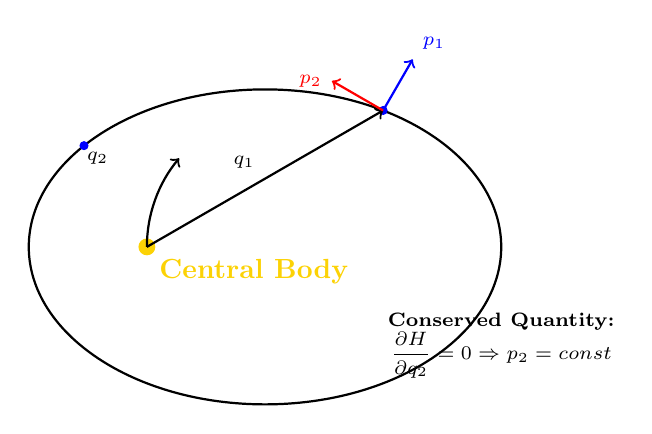
\begin{tikzpicture}[scale=2.5]

  % Draw the orbit path
  \draw[thick] (0,0) ellipse (1.2 and 0.8);

  % Central body
  \filldraw[yellow!70!orange] (-0.6,0) circle (0.04) node[below right=1pt] {\textbf{Central Body}};

  % Orbiting positions
  \foreach \angle in {60, 140} {
    \coordinate (P\angle) at ({1.2*cos(\angle)}, {0.8*sin(\angle)});
    \filldraw[blue] (P\angle) circle (0.02);
  }

  % q1 vector
  \draw[->, thick] (-0.6,0) -- (P60) node[midway, above left] {\scriptsize $q_1$};

  % p1 vector (radial momentum)
  \draw[->, blue, thick] (P60) -- ++(60:0.3) node[above right] {\scriptsize $p_1$};

  % p2 vector (angular momentum)
  \draw[->, red, thick] (P60) -- ++(150:0.3) node[left] {\scriptsize $p_2$};

  % Label q2 arc
  \draw[->, thick] (-0.6,0) arc[start angle=180, end angle=140, radius=0.7];
  \node at (-0.85,0.45) {\scriptsize $q_2$};

  % Conserved quantity box
  \node[align=center] at (1.2,-0.5) {
    \scriptsize \textbf{Conserved Quantity:} \\
    \scriptsize $\displaystyle \frac{\partial H}{\partial q_2} = 0 \Rightarrow p_2 = \text{const}$
  };

\end{tikzpicture}
\caption{Hamiltonian formulation: motion is described by generalized coordinates $q_i$ and conjugate momenta $p_i$. When $q_2$ is absent from $H$, the momentum $p_2$ is conserved—expressing Kepler’s Second Law in Hamilton’s language.}
\end{figure}



Here:

\subsubsection{\( q_1 \): Radial Distance from a Central Body} 
    This coordinate tells us how far the object (like a planet or satellite) is from the center of attraction — such as the Sun. It captures the “in and out” motion, measuring how stretched the orbit is at any given moment.
    
    \begin{figure}[H]
\centering
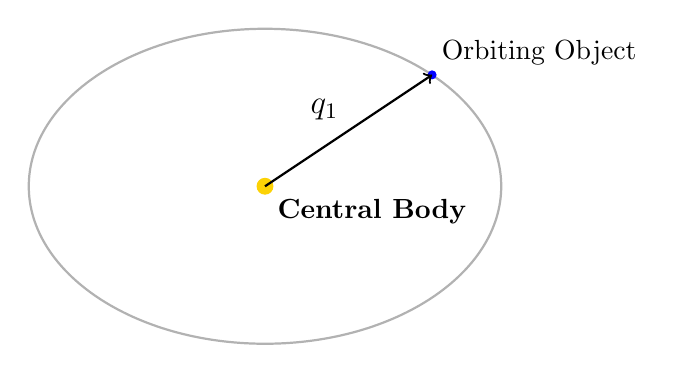
\begin{tikzpicture}[scale=2.5]

  % Central body
  \filldraw[yellow!70!orange] (0,0) circle (0.04);
  \node[below right=1pt] at (0,0) {\textbf{Central Body}};

  % Orbit path (only partial to focus on q1)
  \draw[thick,gray!60] (0,0) ellipse (1.2 and 0.8);

  % Orbiting object
  \coordinate (P) at ({1.2*cos(45)}, {0.8*sin(45)});
  \filldraw[blue] (P) circle (0.02);
  \node[above right] at (P) {Orbiting Object};

  % Radial vector q1
  \draw[->, thick] (0,0) -- (P) node[midway, above left] {\large $q_1$};

\end{tikzpicture}
\caption{\( q_1 \) represents the radial distance from a central body to an orbiting object. It describes the “in and out” motion—how far the object is from the source of attraction at any given time.}
\end{figure}


\subsubsection{\( q_2 \): Angular Coordinate (Still Abstract)} 
    This tracks the direction of the object as it orbits around the center, though we don’t need to tie it to a specific angle like \( \theta \). It simply represents the object’s position along its orbital path — a way of sweeping out the curve over time.


\begin{figure}[H]
\centering
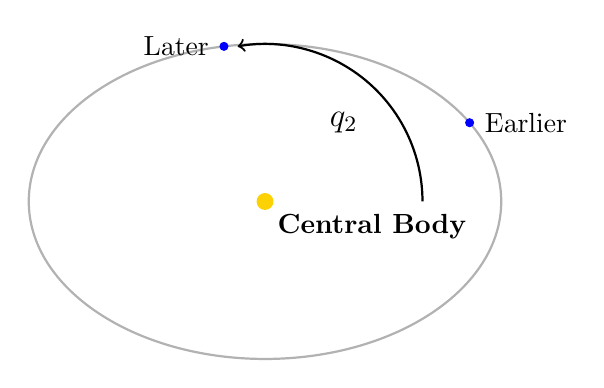
\begin{tikzpicture}[scale=2.5]

  % Central body
  \filldraw[yellow!70!orange] (0,0) circle (0.04);
  \node[below right=1pt] at (0,0) {\textbf{Central Body}};

  % Orbit path
  \draw[thick,gray!60] (0,0) ellipse (1.2 and 0.8);

  % Two orbiting positions
  \coordinate (A) at ({1.2*cos(30)}, {0.8*sin(30)});
  \coordinate (B) at ({1.2*cos(100)}, {0.8*sin(100)});
  \filldraw[blue] (A) circle (0.02);
  \filldraw[blue] (B) circle (0.02);

  \node[right=2pt] at (A) {Earlier};
  \node[left=2pt] at (B) {Later};

  % Angular arc indicating q2
  \draw[->, thick] (0.8,0) arc[start angle=0, end angle=100, radius=0.8];
  \node at (0.4,0.4) {\large $q_2$};

\end{tikzpicture}
\caption{\( q_2 \) represents the angular coordinate — the position along the orbital path. It tracks how the object sweeps through its orbit over time, without needing to be tied to a specific angle like \( \theta \).}
\end{figure}


\subsubsection{\( p_1 \): Momentum Conjugate to \( q_1 \)} 
    This is the momentum associated with radial motion. If the object is moving closer to or farther from the central body, \( p_1 \) increases or decreases accordingly. It’s not just velocity — it’s adjusted for the system’s mass and energy, making it the precise “partner” to \( q_1 \) in phase space.


\begin{figure}[H]
\centering
\begin{tikzpicture}[scale=2.5]

  % Central body
  \filldraw[yellow!70!orange] (0,0) circle (0.04);
  \node[below right=1pt] at (0,0) {\textbf{Central Body}};

  % Orbit path
  \draw[thick,gray!60] (0,0) ellipse (1.2 and 0.8);

  % Orbiting object
  \coordinate (P) at ({1.2*cos(45)}, {0.8*sin(45)});
  \filldraw[blue] (P) circle (0.02);
  \node[above right] at (P) {Orbiting Object};

  % Radial vector (q1)
  \draw[dashed] (0,0) -- (P);

  % Radial momentum vector (p1)
  \draw[->, thick,blue] (P) -- ++(45:0.3);
  \node[above right] at ($(P) + (45:0.3)$) {\large $p_1$};

\end{tikzpicture}
\caption{\( p_1 \) is the momentum conjugate to \( q_1 \), representing motion along the radial direction. It increases or decreases as the object moves closer or farther from the central body, making it the exact momentum "partner" to \( q_1 \) in phase space.}
\end{figure}


\subsubsection{\( p_2 \): Momentum Conjugate to \( q_2 \)} 
    This is the angular momentum — the quantity that tells us how fast and with how much “rotational effort” the object is moving around the center. Just like \( p_1 \) pairs with distance, \( p_2 \) pairs with angle, forming a dynamic duo in the geometry of motion.


\begin{figure}[H]
\centering
\begin{tikzpicture}[scale=2.5]

  % Central body
  \filldraw[yellow!70!orange] (0,0) circle (0.04);
  \node[below right=1pt] at (0,0) {\textbf{Central Body}};

  % Orbit path
  \draw[thick,gray!60] (0,0) ellipse (1.2 and 0.8);

  % Orbiting object
  \coordinate (P) at ({1.2*cos(45)}, {0.8*sin(45)});
  \filldraw[blue] (P) circle (0.02);
  \node[above right] at (P) {Orbiting Object};

  % Tangent vector (angular momentum direction)
  \draw[->, thick,red] (P) -- ++(135:0.3);
  \node[left=3pt] at ($(P) + (135:0.3)$) {\large $p_2$};

\end{tikzpicture}
\caption{\( p_2 \) is the angular momentum — the momentum conjugate to the angular coordinate \( q_2 \). It captures how fast and forcefully the object is rotating around the central body. Like a spinning weight on a string, it reflects the “rotational effort” in the system.}
\end{figure}


\subsubsection{If \( H \) Doesn’t Depend on \( q_2 \), Then \( p_2 \) Is Conserved} 
    This is a key insight from Hamiltonian mechanics. If the Hamiltonian (which describes the total energy of the system) has no explicit dependence on \( q_2 \), it means the system has rotational symmetry — the laws of motion look the same no matter what direction you’re facing. In that case, \( p_2 \) — the angular momentum — remains constant over time. This is a precise, modern way of expressing Kepler’s Second Law: equal areas are swept out in equal times because the angular momentum is conserved.


\begin{figure}[H]
\centering
\begin{tikzpicture}[scale=2.5]

  % Central body
  \filldraw[yellow!80!orange] (0,0) circle (0.04);
  \node[below right=1pt] at (0,0) {\textbf{Central Body}};

  % Orbit path
  \draw[thick,gray!60] (0,0) ellipse (1.2 and 0.8);

  % Two positions on the orbit
  \coordinate (A) at ({1.2*cos(30)}, {0.8*sin(30)});
  \coordinate (B) at ({1.2*cos(110)}, {0.8*sin(110)});
  \filldraw[blue] (A) circle (0.02);
  \filldraw[blue] (B) circle (0.02);

  % Sweep areas (Kepler's equal areas)
  \fill[blue!20,opacity=0.6] (0,0) -- (A) arc[start angle=30,end angle=110,x radius=1.2,y radius=0.8] -- cycle;
  \node at (0.2,0.6) {\scriptsize Equal Area};

  % Angular momentum vector
  \draw[->, thick,red] (A) -- ++(120:0.3);
  \node[above left] at ($(A)+(120:0.3)$) {\large $p_2$};

  % Symmetry indicator
  \draw[->, gray, dashed] (0,0) arc[start angle=0, end angle=360, radius=0.25];
  \node[gray] at (0.4,-0.1) {\scriptsize Symmetry in \( q_2 \)};

\end{tikzpicture}
\caption{If the Hamiltonian has no dependence on \( q_2 \), then \( p_2 \) — the angular momentum — is conserved. This reflects a rotational symmetry in the system, and corresponds to Kepler’s Second Law: equal areas are swept in equal times.}
\end{figure}




\subsection{Conclusion: The Law of Equal Areas, Seen Three Ways}

Kepler’s Second Law began as an empirical observation — a beautifully simple statement: planets sweep out equal areas in equal times. But over the centuries, this idea has been seen through deeper and more abstract lenses, each adding new meaning without changing the core truth.

\begin{itemize}
  \item \textbf{Newton} proved it with geometry and force. He imagined a planet pulled by gravity, moving under the constant tug of the Sun, and used the geometry of triangles to show how area is conserved. In his hands, the law emerged from mechanics — a product of inertia and attraction.

  \item \textbf{Lagrange} reimagined it through symmetry. He didn’t need forces or triangles — only coordinates and invariance. By choosing generalized coordinates and recognizing that the Lagrangian didn’t depend on angle, he uncovered angular momentum as a conserved quantity. The law of equal areas became not a mechanical fact, but a consequence of structure.

  \item \textbf{Hamilton} took it one step further — into geometry itself. In phase space, the planet’s motion became a graceful, volume-preserving flow. The conservation of angular momentum wasn’t just a result — it was a built-in feature of the space through which the system evolves. The law of equal areas was no longer just about motion; it was about the shape of the underlying reality.
\end{itemize}

Each approach offers a different lens on the same truth:  
From Newton’s force, to Lagrange’s symmetry, to Hamilton’s geometry.  
Each one strips away the scaffolding of diagrams and reveals a deeper layer of the cosmos.  

And yet, despite the abstraction, the outcome is the same:  
A planet, tracing its orbit, sweeping out equal areas in equal times — obeying a rhythm not just written in the stars, but etched into the very logic of mathematical physics.

\subsection{Hamilton and the Dot Product: Measuring Flow and Direction}

Before Hamilton gave us his elegant reformulation of mechanics, he made another profound contribution—one that quietly underpins how we understand direction, flow, and change across all of modern science:  
\textbf{the dot product.}

\subsubsection*{Why Invent a New Product?}

In the early 19th century, the idea of multiplying vectors didn’t really exist—not in the clean, directional sense we know today. Scalars could be multiplied. So could polynomials. But what did it mean to “multiply” two directions?

\medskip

Hamilton was searching for a way to describe not just how fast something was moving, but how its motion \textit{aligned} with something else—like a force, a surface, or a path.

He wanted to answer questions like:

\begin{quote}
\textit{How much of a motion points in a given direction?}  
\textit{How does motion project onto constraint?}  
\textit{When are two changes “in step” versus “opposed”?}
\end{quote}

\textbf{His solution was the scalar (dot) product.}

Given two vectors \( \vec{a} \) and \( \vec{b} \), Hamilton defined their scalar product as:
\[
\vec{a} \cdot \vec{b} = \|\vec{a}\| \, \|\vec{b}\| \cos\theta
\]

This definition didn’t just give a number—it gave meaning. It told you how much of \( \vec{a} \) “points in the direction of” \( \vec{b} \). If they were perpendicular, the result was zero. If they pointed the same way, it was maximal.

\subsubsection*{Why This Matters}

Hamilton introduced this tool in the context of \textbf{quaternions}—his ambitious attempt to extend complex numbers into three dimensions. But the dot product took on a life of its own. It became a way to:

\begin{itemize}
    \item Project one motion onto another
    \item Measure alignment or orthogonality
    \item Define energy, work, and change in physical systems
    \item Quantify gradients—how something changes along a direction
\end{itemize}

\begin{tcolorbox}[colback=blue!5!white, colframe=blue!50!black, title={Sidebar: Hamilton's Hidden Legacy—A Geometry of Change}]
Hamilton’s dot product wasn’t just a new kind of multiplication—it was a way to \textbf{measure influence and alignment}.  
This idea became essential in fields like:

\begin{itemize}
    \item \textbf{Mechanics:} Work = force \(\cdot\) displacement
    \item \textbf{Geometry:} Orthogonality = zero dot product
    \item \textbf{Optimization:} Gradients point where dot product is maximized
    \item \textbf{Machine Learning:} Every update in gradient descent is a dot product
\end{itemize}

At its core, the dot product asks: \emph{What direction matters most for change?}
\end{tcolorbox}

\subsubsection*{A Bridge to Optimization}

In the same way that Hamiltonian mechanics let us track how a system flows through space and time, the dot product let us track how a function changes when we move in a particular direction.

This is the heart of \textbf{gradient descent}—an algorithm that finds the direction of steepest decrease in a function by following the negative gradient. It works because:

\[
\text{Change in function} \approx \vec{\nabla}f \cdot \vec{v}
\]

That dot product tells us how much the function \( f \) changes if we move in direction \( \vec{v} \). When that product is large and negative, the function drops quickly. When it’s zero, we’re moving tangent to the level curve—no change.

\medskip

So even here, in the heart of 19th-century physics, Hamilton quietly gave us the tool that would later guide 21st-century algorithms.

\begin{quote}
\textit{He invented the geometry of descent—long before machines ever learned how to learn.}
\end{quote}
